\documentclass[11pt]{article}
\usepackage[english]{babel}
\usepackage[utf8x]{inputenc}
\usepackage{amsmath}
\usepackage{graphicx}
\usepackage[colorinlistoftodos]{todonotes}
\usepackage{listings}
\usepackage[hmargin=2cm]{geometry}
\usepackage{color} 
\definecolor{codegreen}{rgb}{0,0.6,0}
\definecolor{codegray}{rgb}{0.5,0.5,0.5}
\definecolor{codepurple}{rgb}{0.58,0,0.82}
\definecolor{backcolour}{rgb}{0.95,0.95,0.92} 
\lstdefinestyle{mystyle}{
    backgroundcolor=\color{backcolour},   
    commentstyle=\color{codegreen},
    keywordstyle=\color{magenta},
    numberstyle=\tiny\color{codegray},
    stringstyle=\color{codepurple},
    basicstyle=\footnotesize,
    breakatwhitespace=false,         
    breaklines=true,                 
    captionpos=b,                    
    keepspaces=true,                 
    numbers=left,                    
    numbersep=5pt,                  
    showspaces=false,                
    showstringspaces=false,
    showtabs=false,                  
    tabsize=2
}
\lstset{style=mystyle}
\begin{document}
\begin{titlepage}
\newcommand{\HRule}{\rule{\linewidth}{0.5mm}}
\center
\textsc{\LARGE Universidad de Granada}\\[1.5cm] % Name of your university/college
\textsc{\Large Algorítmica}\\[0.5cm] % Major heading such as course name
\textsc{\large Memoria de Prácticas}\\[0.5cm] % Minor heading such as course title
\HRule \\[0.4cm]
{ \huge \bfseries Práctica II: Divide y Vencerás}\\[0.4cm] % Title of your document
\HRule \\[1.5cm]
\begin{minipage}{0.4\textwidth}
\begin{flushleft} \large
\emph{Autores:}\\
Antonio Gámiz Delgado\textsc{} % Your name
\end{flushleft}
\end{minipage}
~
\begin{minipage}{0.4\textwidth}
\begin{flushright} \large
\emph{} \\
\textsc{} % Supervisor's Name
\end{flushright}
\end{minipage}\\[2cm]
{\large 17 de Marzo}\\[2cm] % Date, change the \today to a set date if you want to be precise

\includegraphics{logo.png}\\[1cm]
\vfill % Fill the rest of the page with whitespace
\end{titlepage}

\section{Problema y Objetivo}
Dado un vector de enteros, de tamaño n, ordenado y sin elementos repetidos. Queremos encontrar, si lo hay, una posición $i$ del vector tal que su valor sea igual a ella misma, es decir, que cumpla que $v[i]=i$.
Primero vamos a abordar el problema a lo bruto, y luego aplicaremos la técnica de Divide y Vencerás para ver que este último es más eficiente.
Por último adaptaremos el algoritmo para vectores con elementos repetidos.

\section{Elementos distintos}
\subsection{A lo bruto}
La primera opción que abordamos es la primera que se nos ocurre: recorrer el vector $v$ desde $0$ hasta $n-1$ y parar cuando encontremos el primer elemento que cumple la condición.
Por lo que nos queda el siguiente código:

\begin{lstlisting}[language=C]
int algoritmo_bruto(vector<int> v)
{
  for(int i=0; i<v.size(); i++){
    if(v[i]==i) return i;
  }
  return -1;
}
\end{lstlisting}

Evidentemente el análisis de la eficiencia de este algoritmo nos da un orden lineal, es decir, $T(n)=n$.

De forma empírica comprobamos que efectivamente tenemos:

\begin{figure}[h]
\centering
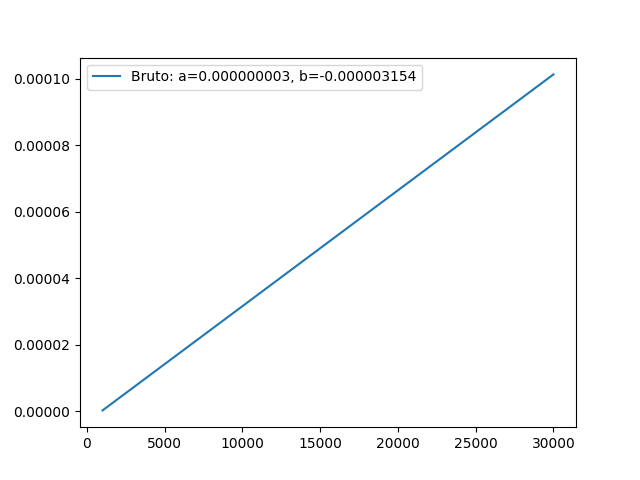
\includegraphics[scale=0.5]{../graphics/bruto_def.png}
\end{figure}

\newpage

\subsection{Divide y vencerás(sin repeticiones)}

Como el vector con el que estamos trabajando, $v$, está ordenado de menor a mayor (orden creciente), parece razonable pensar en un algoritmo parecido a la búsqueda binaria, fijándonos en el elemento que se encuentra en el medio del vector, $m=\frac{n}{2}$. Si este número coincide con el valor de $v[m]$, entonces hemos terminado. 

En caso contrario, hay dos posibilidades: $v[m]>m$ o $v[m]<m$. Estudiamos el primer caso y el otro es análogo. Por lo que si tenemos que $v[m]>m$, al estar los elementos ordenados y sin repetición, sabemos que para todos los índices $i$ mayores que que $m$, los valores en esas posiciones, $v[i]$, serán siempre mayores que $v[m]$, es decir, $v[i]>i \quad \forall i > m$. Por tanto, sabemos que a la derecha de $m$ no se puede dar la situación que buscamos, luego nos la "saltamos" en el algoritmo, es decir, reducimos la búsqueda a la otra parte del vector, a la izquierda de $m$. El otro caso se razona de forma análoga.

Por lo que nos queda el siguiente algoritmo recursivo:
\begin{lstlisting}[language=C]
int divide_nr(vector<int>& v, int n1, int n2)
{
  if( n1==n2 )
    if( v[n1]==n1 ) return n1;
  else return -1;
  else {
    int middle=(n1+n2)/2;
    if( v[middle]==middle ) return middle;
    else if ( v[middle] > middle ) return divide_nr(v, n1, middle-1);
    else return divide_nr(v, middle+1, n2);
  }
}
\end{lstlisting}

El tiempo de ejecución del algoritmo viene dado por la expresión $T(n)=T(\frac{n}{2})+a$. Con el cambio de variable $t_k=T(2k)$, tenemos que $t_k-t_{k-1}-a=0$. Es una ecuación en recurrencia no homogénea con ecuación característica $(x-1)^2=0$. Resolviéndola obtenemos que $t_k=c_1k+c_2$ y deshaciendo el cambio de variable anterior ($n=2k$) nos queda que $T(n)=c_1\log n+c_2\in O(\log n)$ 

De forma empírica comprobamos que efectivamente tenemos:

\newpage

\begin{figure}[h]
\centering
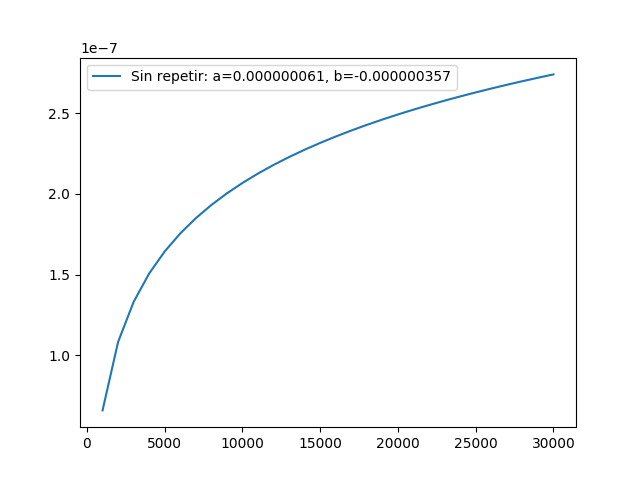
\includegraphics[scale=0.5]{../graphics/sin_repetir_def.png}
\caption{Eficiencia empirica}
\end{figure}


\begin{figure}[h]
\centering
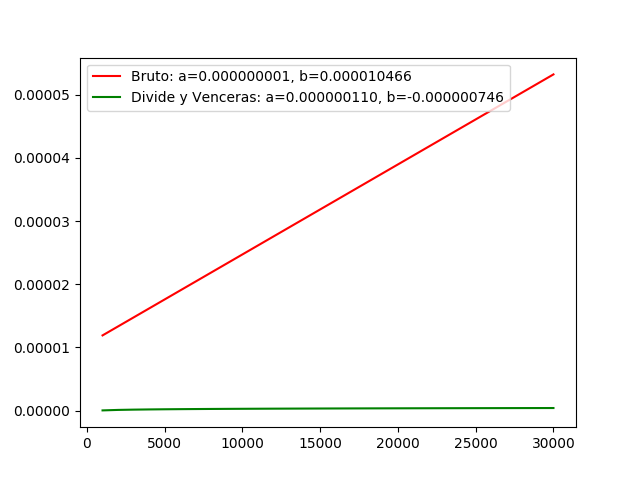
\includegraphics[scale=0.5]{../graphics/juntas_def.png}
\caption{Empiciencia empírica de Fuerza Bruta y Divide y vencerás}
\end{figure}


\newpage

\subsection{Divide y vencerás (con repeticiones)}

En este caso el algoritmo anterior no funcionará en algunos casos ya que el razonamiento usado anteriormente no es válido (necesitamos la desigualdad estricta, y en este caso no contamos con ella).
Por lo que en este caso no podemos descartar de forma segura una de las partes del vector, pero lo que sí podemos asegurar en este caso es que, si $v[m]>m$, entonces para ningún índice $j$ situado entre los índices $m$ y $v[m]$ se cumple $v[j]=j$. Esto es así porque para cualquier $j$ en ese rango se tiene que $v[j]\geq v[m]>j$.

Por tanto nos centramos en dos rangos, $(1,m)$ y $(v[m], n)$. Ahora, el razonamiento es análogo al anterior pero con estos nuevos rangos. Quedando el siguiente algoritmo recursivo un poco más complejo:
\begin{lstlisting}[language=C]
int divide_r(vector<int>& v, int n1, int n2){
  if( n1==n2 ){
    if( v[n1]==n1 ) 
      return n1;
    else 
      return -1;
  }else{
    int middle=(n1+n2)/2;
    if( v[middle]==middle ) 
      return middle;
    else if( v[middle] > middle ){
      
      int left=divide_r(v, n1, middle-1);
      int right;
      
      if( v[middle] <= n2 ) 
        right=divide_r(v, v[middle], n2);
      else right=0;

      if( left!=0 ) return left;
      if( right!=0 ) return right;
      
      return -1;
    }else{
      int right=divide_r(v, middle+1, n2);
      int left;

      if( n1<=v[middle] ) left=divide_r(v, n1, v[middle]);
      else left=0;

      if( right!=0 ) return right;
      if( left!=0 ) return left;

      return -1;
    }
  }
}
\end{lstlisting}

\section{Capturas}
Adjunto algunas capturas para ver el correcto funcionamiento del algoritmo:

\begin{figure}[h]
\centering
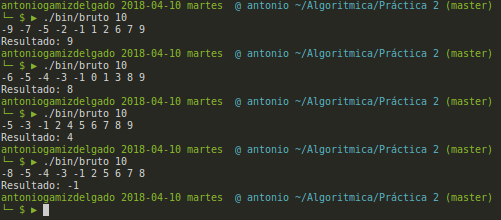
\includegraphics[scale=0.4]{../graphics/bruto_c.png}
\caption{Algoritmo Bruto}
\end{figure}

\begin{figure}[h]
\centering
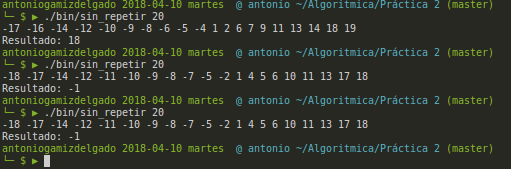
\includegraphics[scale=0.4]{../graphics/sin_repe_c.png}
\caption{Divide y vencerás (sin repetición)}
\end{figure}

\begin{figure}[h]
\centering
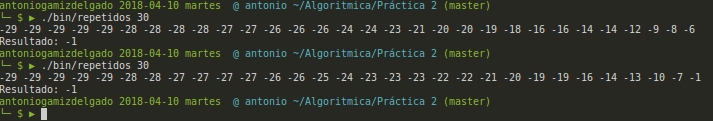
\includegraphics[scale=0.4]{../graphics/repe_c.png}
\caption{Divide y vencerás (con repetición)}
\end{figure}


\end{document}